% -*- root: ../../../thesis.tex -*-

\section[A complete reproducible workflow]{\texorpdfstring{A complete reproducible workflow - From a\\species list to a phylogeny, and\\distribution map.}{A complete reproducible workflow - From a species list to a phylogeny, and distribution map.}} 
\label{ap:taxize:one} 

If you aren't familiar with a complete workflow in R, it may be difficult to visualize the process. In R, everything is programmatic, so the whole workflow can be in one place, and be repeated whenever necessary. The following is a workflow for taxize, going from a species list to a phylogeny. 

First, install taxize

\begin{knitrout}
\color{fgcolor}\small\begin{kframe}
\begin{alltt}
\hlstd{R> }\hlkwd{install.packages}\hlstd{(}\hlstr{"taxize"}\hlstd{)}
\end{alltt}
\end{kframe}
\end{knitrout}


Then load it into R

\begin{knitrout}
\color{fgcolor}\small\begin{kframe}
\begin{alltt}
\hlstd{R> }\hlkwd{library}\hlstd{(taxize)}
\end{alltt}
\end{kframe}
\end{knitrout}


Most of us will start out with a species list, something like the one below. Note that each of the names is spelled incorrectly.

\begin{knitrout}
\color{fgcolor}\small\begin{kframe}
\begin{alltt}
\hlstd{R> splist} \hlkwb{<-} \hlkwd{c}\hlstd{(}\hlstr{"Helanthus annuus"}\hlstd{,} \hlstr{"Pinos contorta"}\hlstd{,} 
                \hlstr{"Collomia grandiflorra"}\hlstd{,} \hlstr{"Rosa california"}\hlstd{,}
                \hlstr{"Mimulus bicolour"}\hlstd{,} \hlstr{"Nicotiana glauca"}\hlstd{,} \hlstr{"Maddia sativa"}\hlstd{)}
\end{alltt}
\end{kframe}
\end{knitrout}


There are many ways to resolve taxonomic names in taxize. Of course, the ideal name resolver will do the work behind the scenes for you so that you don't have to do things like fuzzy matching. There are a few services in taxize like this we can choose from: the Global Names Resolver service from EOL (see function \emph{gnr\_resolve}) and the Taxonomic Name Resolution Service from iPlant (see function \emph{tnrs}). In this case let's use the function \emph{tnrs}. 

\begin{knitrout}
\color{fgcolor}\small\begin{kframe}
\begin{alltt}
\hlcom{# The tnrs function accepts a vector of 1 or more}
\hlstd{R> splist_tnrs} \hlkwb{<-} \hlkwd{tnrs}\hlstd{(}\hlkwc{query} \hlstd{= splist,} \hlkwc{getpost} \hlstd{=} \hlstr{"POST"}\hlstd{,} 
                        \hlkwc{source_} \hlstd{=} \hlstr{"iPlant_TNRS"}\hlstd{)}
\hlcom{# Remove some fields}
\hlstd{R> (splist_tnrs} \hlkwb{<-} \hlstd{splist_tnrs[,} \hlopt{!}\hlkwd{names}\hlstd{(splist_tnrs)} \hlopt 
                        \hlkwd{c}\hlstd{(}\hlstr{"matchedName"}\hlstd{,} \hlstr{"annotations"}\hlstd{,}
                        \hlstr{"uri"}\hlstd{)])}
\end{alltt}
\begin{verbatim}
#           submittedName         acceptedName    sourceId score
# 5      Helanthus annuus    Helianthus annuus iPlant_TNRS  0.98
# 1        Pinos contorta       Pinus contorta iPlant_TNRS  0.96
# 7 Collomia grandiflorra Collomia grandiflora iPlant_TNRS  0.99
# 6       Rosa california     Rosa californica iPlant_TNRS  0.99
# 4      Mimulus bicolour      Mimulus bicolor iPlant_TNRS  0.98
# 3      Nicotiana glauca     Nicotiana glauca iPlant_TNRS     1
# 2         Maddia sativa         Madia sativa iPlant_TNRS  0.97
\end{verbatim}
\begin{alltt}
\hlcom{# Note the scores. They suggest that there were no perfect matches,}
\hlcom{# but they were all very close, ranging from 0.77 to 0.99}
\hlcom{# (1 is the highest).}
\hlcom{# Let's assume the names in the 'acceptedName' column}
\hlcom{# are correct (and they should}
\hlcom{# be).}
\hlcom{# So here's our updated species list}
\hlstd{R> (splist} \hlkwb{<-} \hlkwd{as.character}\hlstd{(splist_tnrs}\hlopt{$}\hlstd{acceptedName))}
\end{alltt}
\begin{verbatim}
# [1] "Helianthus annuus"  "Pinus contorta"  "Collomia grandiflora"
# [4] "Rosa californica"  "Mimulus bicolor"  "Nicotiana glauca"    
# [7] "Madia sativa"
\end{verbatim}
\end{kframe}
\end{knitrout}


Another thing we may want to do is collect common names for our taxa. 

\begin{knitrout}
\color{fgcolor}\small\begin{kframe}
\begin{alltt}
\hlstd{R> tsns} \hlkwb{<-} \hlkwd{get_tsn}\hlstd{(}\hlkwc{searchterm} \hlstd{= splist,} \hlkwc{searchtype} \hlstd{=} \hlstr{"sciname"}\hlstd{,} 
                    \hlkwc{verbose} \hlstd{=} \hlnum{FALSE}\hlstd{)}
\hlstd{R> comnames} \hlkwb{<-} \hlkwd{lapply}\hlstd{(tsns, getcommonnamesfromtsn)}
\hlcom{# Unfortunately, common names are not standardized like species}
\hlcom{# names, so there are multiple common names for each taxon}
\hlstd{R> }\hlkwd{sapply}\hlstd{(comnames, length)}
\end{alltt}
\begin{verbatim}
# [1] 3 3 3 3 3 3 3
\end{verbatim}
\begin{alltt}
\hlcom{# So let's just take the first common name for each species}
\hlstd{R> comnames_vec} \hlkwb{<-} \hlkwd{do.call}\hlstd{(c,} \hlkwd{lapply}\hlstd{(comnames,} 
            \hlkwa{function}\hlstd{(}\hlkwc{x}\hlstd{)} \hlkwd{as.character}\hlstd{(x[}\hlnum{1}\hlstd{,} \hlstr{"comname"}\hlstd{])))}
\hlcom{# And we can make a data.frame of our scientific and common names}
\hlstd{R> (allnames} \hlkwb{<-} \hlkwd{data.frame}\hlstd{(}\hlkwc{spname} \hlstd{= splist,} \hlkwc{comname} \hlstd{= comnames_vec))}
\end{alltt}
\begin{verbatim}
#                 spname                       comname
# 1    Helianthus annuus              common sunflower
# 2       Pinus contorta                lodgepole pine
# 3 Collomia grandiflora        largeflowered collomia
# 4     Rosa californica           California wildrose
# 5      Mimulus bicolor yellow and white monkeyflower
# 6     Nicotiana glauca                  tree tobacco
# 7         Madia sativa                 coast tarweed
\end{verbatim}
\end{kframe}
\end{knitrout}


Another common task is getting the taxonomic tree upstream from your study taxa. We often know what family or order our taxa are in, but it we often don't know the tribes, subclasses, and superfamilies. taxize provides many avenues to getting classifications. Two of them are accessible via a single function (\emph{classification}): the Integrated Taxonomic Information System (ITIS) and National Center for Biotechnology Information (NCBI); and via the Catalogue of Life (see function \emph{col\_classification}):

\begin{knitrout}
\color{fgcolor}\small\begin{kframe}
\begin{alltt}
\hlcom{# As we already have Taxonomic Serial Numbers from ITIS, let's just}
\hlcom{# get classifications from ITIS.Note that we could use uBio instead.}
\hlstd{R> class_list} \hlkwb{<-} \hlkwd{classification}\hlstd{(tsns)}
\hlstd{R> }\hlkwd{sapply}\hlstd{(class_list, nrow)}
\end{alltt}
\begin{verbatim}
# [1] 12 11 12 12 12 12 12
\end{verbatim}
\begin{alltt}
\hlcom{# And we can attach these names to our allnames data.frame}
\hlstd{R> }\hlkwd{library}\hlstd{(plyr)}
\hlstd{R> gethiernames} \hlkwb{<-} \hlkwa{function}\hlstd{(}\hlkwc{x}\hlstd{) \{}
        \hlstd{temp} \hlkwb{<-} \hlstd{x[,} \hlkwd{c}\hlstd{(}\hlstr{"rankName"}\hlstd{,} \hlstr{"taxonName"}\hlstd{)]}
        \hlstd{values} \hlkwb{<-} \hlkwd{data.frame}\hlstd{(}\hlkwd{t}\hlstd{(temp[,} \hlnum{2}\hlstd{]))}
        \hlkwd{names}\hlstd{(values)} \hlkwb{<-} \hlstd{temp[,} \hlnum{1}\hlstd{]}
        \hlkwd{return}\hlstd{(values)}
\hlstd{R> \}}
\hlstd{R> class_df} \hlkwb{<-} \hlkwd{ldply}\hlstd{(class_list, gethiernames)}
\hlstd{R> allnames_df} \hlkwb{<-} \hlkwd{merge}\hlstd{(allnames, class_df,} \hlkwc{by.x} \hlstd{=} \hlstr{"spname"}\hlstd{,} 
                        \hlkwc{by.y} \hlstd{=} \hlstr{"Species"}\hlstd{)}
\hlcom{# Now that we have allnames_df, we can start to see some}
\hlcom{# relationships among species simply by their shared taxonomic names}
\hlstd{R> allnames_df[}\hlnum{1}\hlopt{:}\hlnum{2}\hlstd{, ]}
\end{alltt}
{\small
\begin{verbatim}
#                 spname                comname Kingdom     Subkingdom
# 1 Collomia grandiflora largeflowered collomia Plantae Viridaeplantae
# 2    Helianthus annuus       common sunflower Plantae Viridaeplantae
#   Infrakingdom     Division     Subdivision Infradivision        
# 1 Streptophyta Tracheophyta Spermatophytina  Angiospermae
# 2 Streptophyta Tracheophyta Spermatophytina  Angiospermae 
#   Class         Superorder     Order        Family      Genus
# 1  Magnoliopsida Asteranae  Ericales Polemoniaceae   Collomia
# 2  Magnoliopsida Asteranae Asterales    Asteraceae Helianthus
\end{verbatim}
}
\begin{alltt}

# Ah, so Abies and Bartlettia are in different infradivisions, but 
# share taxonomic names above that point.
\end{alltt}
\end{kframe}
\end{knitrout}


However, taxonomy can only get you so far. Shared ancestry can be reconstructed from molecular data, and phylogenies created. Phylomatic is a web service with an API that we can use to get a phylogeny. 


\begin{knitrout}
\color{fgcolor}\small\begin{kframe}
\begin{alltt}
\hlcom{# Fetch phylogeny from phylomatic}
\hlstd{R> phylogeny} \hlkwb{<-} \hlkwd{phylomatic_tree}\hlstd{(}\hlkwc{taxa} \hlstd{=} \hlkwd{as.character}\hlstd{(allnames}\hlopt{$}\hlstd{spname),} 
            \hlkwc{taxnames} \hlstd{=} \hlnum{TRUE}\hlstd{,}
            \hlkwc{get} \hlstd{=} \hlstr{"POST"}\hlstd{,} \hlkwc{informat} \hlstd{=} \hlstr{"newick"}\hlstd{,} \hlkwc{method} \hlstd{=} \hlstr{"phylomatic"}\hlstd{,} 
            \hlkwc{storedtree} \hlstd{=} \hlstr{"R20120829"}\hlstd{,}
            \hlkwc{taxaformat} \hlstd{=} \hlstr{"slashpath"}\hlstd{,} \hlkwc{outformat} \hlstd{=} \hlstr{"newick"}\hlstd{,} \hlkwc{clean} \hlstd{=} \hlstr{"true"}\hlstd{,} 
            \hlkwc{parallel} \hlstd{=} \hlnum{TRUE}\hlstd{)}
\hlcom{# Format teeth-labels}
\hlstd{R> phylogeny}\hlopt{$}\hlstd{tip.label} \hlkwb{<-} \hlkwd{capwords}\hlstd{(phylogeny}\hlopt{$}\hlstd{tip.label,} 
                         \hlkwc{onlyfirst} \hlstd{=} \hlnum{TRUE}\hlstd{)}
\hlcom{# plot phylogeny}
\hlstd{R> }\hlkwd{plot}\hlstd{(phylogeny)}
\end{alltt}
\end{kframe}\begin{figure}[!ht]


{\centering 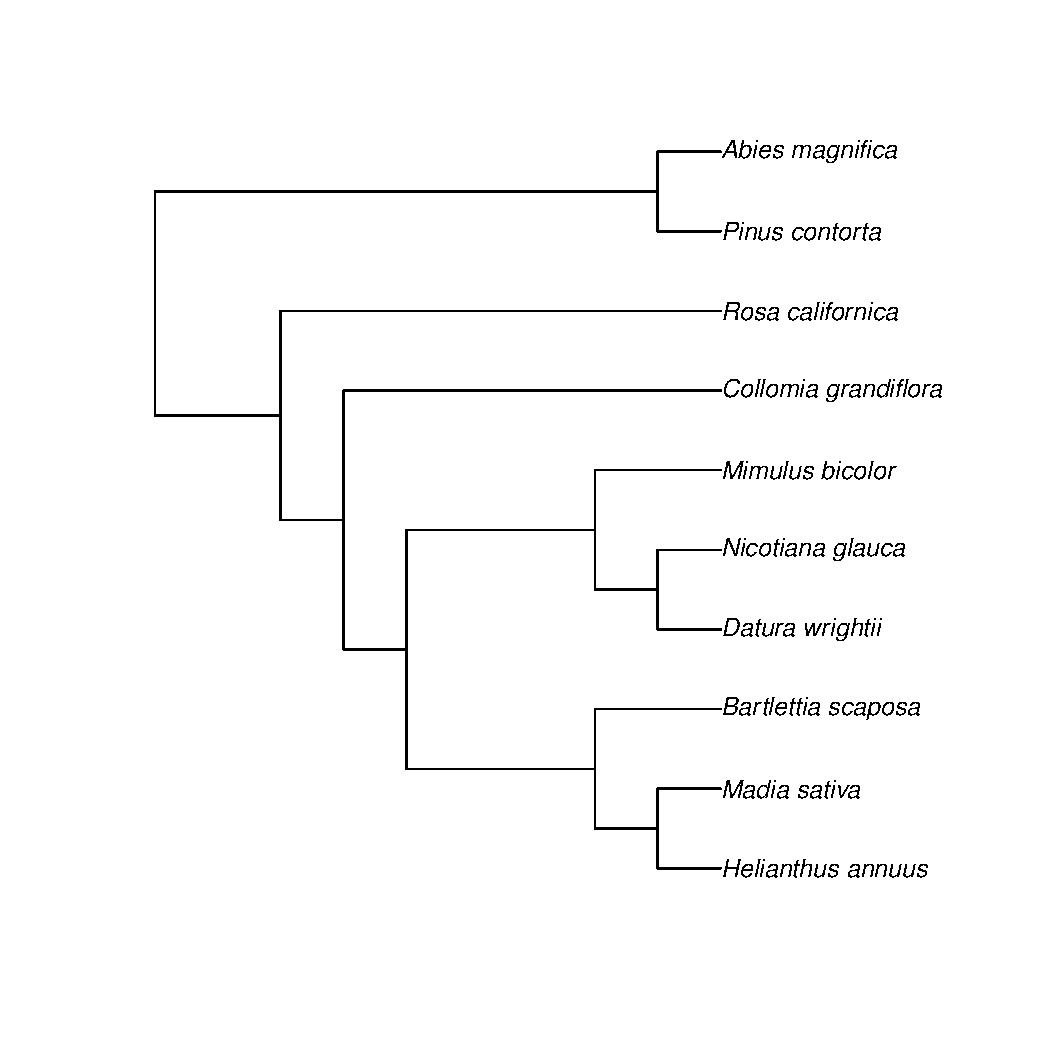
\includegraphics[width=4in,height=4in]{appendix/taxize/one/phylogeny.pdf} 

}

\caption[A phylogeny created using taxize]{A phylogeny created using taxize.\label{fig:phylophylogeny}}
\end{figure}
\end{knitrout}



Using the species list, with the corrected names, we can now search for occurrence data. The Global Biodiversity Information Facility (GBIF) has the largest collection of records data, and has a  API that we can interact with programmatically from R. First, we need to install rgbif.

\begin{knitrout}
\color{fgcolor}\small\begin{kframe}
\begin{alltt}
\hlcom{# Install rgbif from github.com}
\hlstd{R> }\hlkwd{install.packages}\hlstd{(}\hlstr{"devtools"}\hlstd{)}
\hlstd{R> }\hlkwd{library}\hlstd{(devtools)}
\hlstd{R> }\hlkwd{install_github}\hlstd{(}\hlstr{"rgbif"}\hlstd{,} \hlstr{"ropensci"}\hlstd{)}
\end{alltt}
\end{kframe}
\end{knitrout}


Now we can search for occurrences for our species list and make a map.


\begin{knitrout}
\color{fgcolor}\small\begin{kframe}
\begin{alltt}
\hlstd{R> }\hlkwd{library}\hlstd{(rgbif)}
\hlstd{R> }\hlkwd{library}\hlstd{(ggplot2)}
\hlcom{# get occurences}
\hlstd{R> occurr_list} \hlkwb{<-} \hlkwd{occurrencelist_many}\hlstd{(}\hlkwd{as.character}\hlstd{(allnames}\hlopt{$}\hlstd{spname),} 
            \hlkwc{coordinatestatus} \hlstd{=} \hlnum{TRUE}\hlstd{,}
            \hlkwc{maxresults} \hlstd{=} \hlnum{100}\hlstd{,} \hlkwc{removeZeros} \hlstd{=} \hlnum{TRUE}\hlstd{,} 
            \hlkwc{fixnames} \hlstd{=} \hlstr{"changealltorig"}\hlstd{)}
\hlcom{# Make a map}
\hlstd{R> p} \hlkwb{<-} \hlkwd{gbifmap_list}\hlstd{(occurr_list)} \hlopt{+} 
            \hlkwd{guides}\hlstd{(}\hlkwc{col} \hlstd{=} \hlkwd{guide_legend}\hlstd{(}\hlkwc{title} \hlstd{=} \hlstr{""}\hlstd{,} \hlkwc{nrow} \hlstd{=} \hlnum{3}\hlstd{,}
            \hlkwc{byrow} \hlstd{=} \hlnum{TRUE}\hlstd{))} \hlopt{+} \hlkwd{theme}\hlstd{(}\hlkwc{legend.position} \hlstd{=} \hlstr{"bottom"}\hlstd{,} 
            \hlkwc{legend.key} \hlstd{=} \hlkwd{element_blank}\hlstd{())} \hlopt{+}
            \hlkwd{coord_equal}\hlstd{()}
\hlstd{R> p}
\end{alltt}
\end{kframe}\begin{figure}[ht]


{\centering 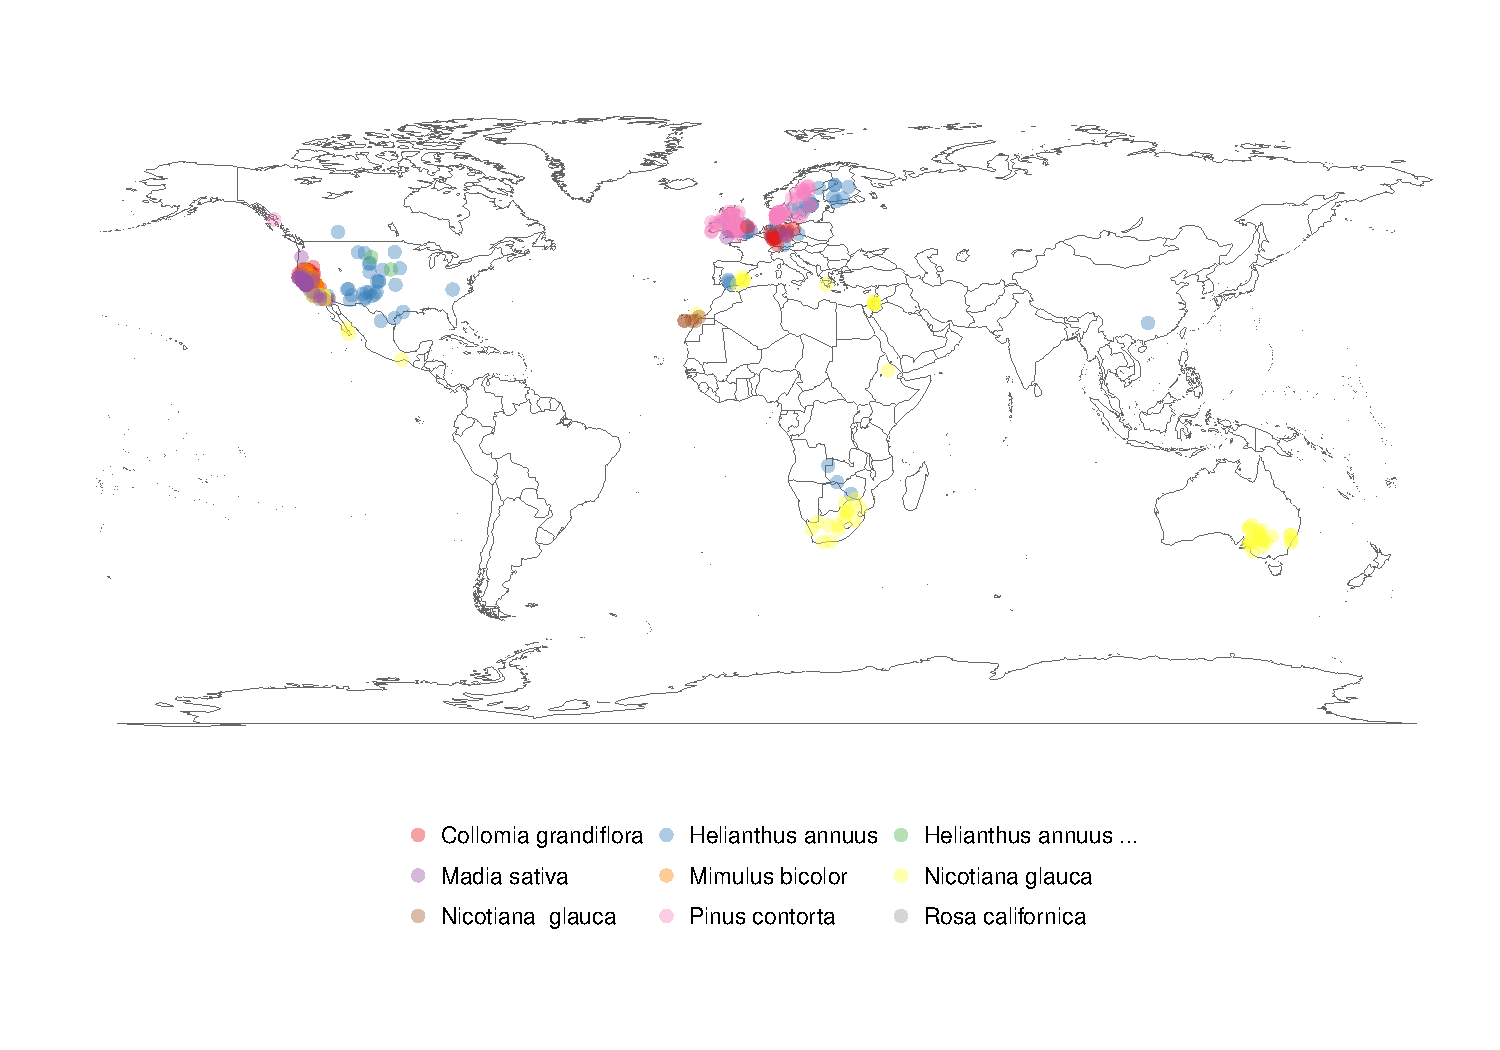
\includegraphics[width=0.9\textwidth]{appendix/taxize/one/plot_map.pdf} 

}

\caption[A map created using taxize]{A map created using taxize.\label{fig:mapplot_map}}
\end{figure}


\end{knitrout}
